\chapter{Literature Review}
\label{chap:lit}
%%%%%%%%%%%%%%%%%%%%%%%%%%%%%%%%%%%%%%%%%%%%%%%%%%%%%%%%%%%%%%%%
%% Literature review for CC

\section{Collaborative Consumption}

\subsection{Defining CC}
\textit{"Collaborative Consumption (CC)"} is people, in a community, acquiring or distributing physical goods or services for \textit{some form of compensation} amongst themselves \cite{Belk:2014}. The form of compensation dictates whether the transaction can be labelled as \textit{Sharing} ownership, \textit{Swapping or Trading} for another resource or even \textit{Buying and Selling} of used goods. One commonality in all such practices is the interaction amongst the community members using technology, especially Web 2.0 (otherwise known as the \textit{interactive Web}). Sharing items within a small organisation like family or friends has been present in society for a very long time, but the technologies like social networks, e-commerce etc. available today allow people to make trusted transactions in large communities. In fact, the CC platforms are merely \textit{"economical-technological coordination providers"} \cite{Hamari:2015}. In other words, people have been willing to engage in 'Sharing Economy' if a suitable technological platform exists.\\

\subsection{CC Categories}
There are three categories of Collaborative Consumption \cite{Albinsson:2012} :

\begin{itemize}

	\item Where consumers pay for using a resource. For example: Singapore based \href{http://www.rent-that-toy.com}{Rent-A-Toy} rents expensive toys for a fee.
	
	\item Where members redistribute their rarely used or unwanted items. For example: \href{http://www.heyneighborapp.com}{Hey, Neighbor!} is a site where those in particular locales can share/rent their equipment and 'micro-favours'.
	
	\item Where people share less tangible resources like skills, space, time etc. For example: \href{https://www.airbnb.co.uk}{Airbnb} and \href{https://www.couchsurfing.com}{Couchsurfing} members temporarily share their living space with fellow members.

\end{itemize}

On the other hand, two categories of Collaborative Consumption exchanges are \cite{Hamari:2015} - 

\begin{itemize}

	\item \textbf{\textit{Access over ownership}}: When a user offers and shares their resources for a limited time to another user in the community (with or without the need for an  exchange). For example: \href{https://www.renttherunway.com}{Rent the Runway} rents expensive designer cloths to people for a fee or \href{https://www.yourparkingspace.co.uk}{Your Parking Space} lets the users to list their parking space to be available to rent to others.
	
	\item \textbf{\textit{Transfer ownership}}: When a user completely relinquishes their claim on an item and gives it away to another (also with or without the need for an  exchange). For example: \href{http://www.swapstyle.com}{Swapstyle} lets its users swap their cloths. 

\end{itemize}

\subsection{Reasons to Participate}
Four possible reasons why people take part in Collaborative Consumption \cite{Hamari:2015} are - 

\begin{itemize}

	\item \textbf{\textit{Sustainability}}: People want to reuse and recycle their owned goods to bring wastage to a minimum and sustain a better environment.
	
	\item \textbf{\textit{Enjoyment}}: Users often enjoy sharing their produced item because it can help others. For example: Many software developers give away their software source code on \href{https://github.com}{Github} because they enjoy software freedom.
	
	\item \textbf{\textit{Reputation}}: Users enjoy the earned reputation in the community from participating in many transactions. For example: Well traded \href{http://www.ebay.co.uk}{Ebay} users usually carry out more successful transactions.
	
	\item \textbf{\textit{Economic Benefits}}: Members want to save some cost by swapping their items, buying used ones or earn some money by selling unwanted goods.
	
\end{itemize}

The followings affect the satisfaction of a sharing option \cite{Mohlmann:2015}-
\begin{itemize}

	\item \textbf{\textit{Cost Savings}}: A sharing option that saves some money for the consumer leads to a successful transaction more often.
	
	\item \textbf{\textit{Familiarity}}: Consumers trade more often on Collaborative Consumption platforms that they are familiar with (through exposure from various media).
	
	\item \textbf{\textit{Service Quality}}: Members use Collaborative Consumption platforms that give them easy options, suggestions and an overall better experience.
	
	\item \textbf{\textit{Trust}}: People only want to carry out transactions if they feel that the community is secure, welcoming and the members are trustworthy.
	
\end{itemize}

\subsection{Collaborative Consumption in UoS}
University of Southampton students also have a Facebook Group called \href{https://www.facebook.com/groups/302702106480967/?fref=ts}{Free \& For Sale}, where students put up their unwanted item to sell, swap or give away. These items can include calculators, books, cloths, fashion accessories, furniture, kitchen tools, garage tools, event tickets, transport tickets, mobiles, laptops, electronic boards etc. Students arrange the transactions within themselves. The group has been quite successful in recent years.\\

The above leads me to believe that University of Southampton students can truly benefit from a Collaborative Consumption platform which lets \textit{only} them trade on the platform and integrates with their campus identity. There are existing platforms including \textbf{Ebay}, \textbf{Gumtree} and \textbf{Facebook} where students can co-ordinate their transactions. But none of these are suited for this particular atmosphere and cannot provide support for a UoS community.

%%%%%%%%%%%%%%%%%%%%%%%%%%%%%%%%%%%%%%%%%%%%%%%%%%%%%%%%%%%%%%%%



%%%%%%%%%%%%%%%%%%%%%%%%%%%%%%%%%%%%%%%%%%%%%%%%%%%%%%%%%%%%%%%%
%% Literature review for Hybrid Dev

\section{Hybrid Mobile Development}

\subsection{Mobile Applications}

\textbf{Native} apps are those built using platform specific tools, for example: Swift or C\# and XCode for iOS, Java (Dalvik runtime) and Android Studio for Android etc. Examples are - Gmail by Google, Pages by Apple etc.\\

\textbf{Web} apps are built using HTML, CSS and JavaScript and hosted on a \textit{website} that can be accessed from any browser including a mobile. Examples are - Netflix website or Google Docs etc.\\

\textbf{Hybrid} apps sit between native and web apps (Figure \ref{Figure:Hybrid} \cite{salesforcehybrid-site}). They are built using similar technologies as web apps, but are then compiled into platform specific installers and used as a native app. Underneath the surface, these apps usually run a \textit{localhost} server on the mobile that runs the app and the OS accesses them using web-view. \cite{Litayem:2015, Karadimce:2014}

\begin{figure}[!h]
  \centering
    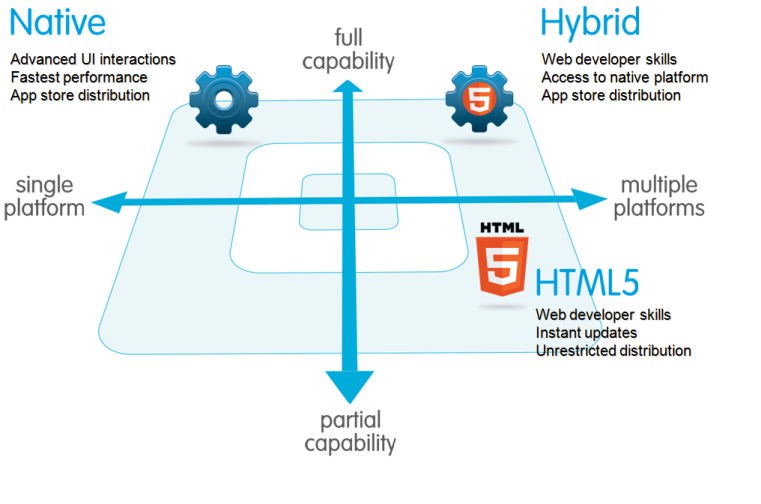
\includegraphics[width=0.6\textwidth]{hybrid-a}
  	\caption{Hybrid Apps}
  \label{Figure:Hybrid}
\end{figure}

\subsection{Advantages of Hybrid Apps}

A major difficulty in native development is that, it easily becomes difficult to simultaneously develop, maintain and support for different platforms \cite{Litayem:2015}. Very little of one device's code can be ported over to another because of lack of standards, e.g. the standard Android uses commas to separate items in a list, but Samsung phones use a semicolon \cite{Joorabchi:2013}. Whereas, a hybrid app can be ported into multiple platforms simultaneously, with very little (if any) change.\\

Native apps usually perform better than their web and hybrid counterparts because they can leverage the full potential of the OS. While web apps have a disadvantage of being accessible only over network and are slow to respond, recent hybrid app development frameworks have started hardware acceleration. In fact, apart from 3D games, there is negligible or unnoticeable performance gap between the two paradigms \cite{Charland:2011}.\\

Early web and hybrid apps were notorious for their lack of usability on a mobile, because the components such as buttons were not optimised for touch. Modern frameworks, however, provide the exact components as the native apps. Resultantly "end users value hybrid and native apps similarly" \cite{Malavolta:2015}.

\subsection{Challenges in Hybrid Apps}

Lack of automated testing frameworks is a major drawback for production ready hybrid apps. The mobile app industry, in general, does not have a unified testing pattern for either usability or functional testing \cite{Joorabchi:2013}. Each OS provider has its own IDE (Integrated Development Environment) and test environment. But most hybrid frameworks, being very recent and open-source, do not have such features.\\

Moreover, debugging is difficult in mobile apps, in general, because CPU, memory etc. monitoring is cumbersome, even impossible at times. This is specially true in hybrid frameworks, as most only support primitive emulation rather than a debugger.\\

Finally, security is an emerging issue. Being built on web technologies, it is subject to threats from that paradigm as well as mobile OS threats \cite{Brucker:2016, Hale:2015}.\\

Nevertheless, I believe hybrid technologies are perfect for a short project with intentions of fast prototyping and user evaluation.

%%%%%%%%%%%%%%%%%%%%%%%%%%%%%%%%%%%%%%%%%%%%%%%%%%%%%%%%%%%%%%%%



%%%%%%%%%%%%%%%%%%%%%%%%%%%%%%%%%%%%%%%%%%%%%%%%%%%%%%%%%%%%%%%%
%% Literature review for Scrum

\section{Agile Development \& Scrum}

\subsection{Overview of Agile Method}

The “Agile Manifesto" \cite{beck:2001} stated four core principles - 

\begin{enumerate}
	\item \textbf{Individuals and interactions} over processes and tools
	\item \textbf{Working software} over comprehensive documentation
	\item \textbf{Customer collaboration} over contract negotiation
	\item \textbf{Responding to change} over following a plan
\end{enumerate}

Put simple, agile software development is to - define a vision and scope for the project, define requirements together with customer, build in iterations and review the results with the customer to update the requirements until release \cite{Inayat:2015}. This iterative framework is called \textbf{Scrum}.

\subsection{Scrum}

In Scrum framework, the development team works closely with the \textbf{Product Owner} (usually the customer). The team defines requirements in forms of \textbf{User Stories} (\texttt{As a <user>, I want <feature> so that <reason>} \cite{Rees:2002}); how the task is carried out is left open. The project is broken down into iterations (typically 1-4 weeks), each with a goal such that the vision of the project is fulfilled by the release period \cite{Schwaber:1997}.\\

The long list of tasks is called the \textbf{Product Backlog}. At each iteration, tasks are selected (\textbf{Sprint Backlog}) to generate a \textit{working} software of \textit{value} to the customer. This is then demonstrated to the product owner and shippability is discussed. Backlog is updated and prioritised with possibly new or reduced items (Figure \ref{Figure:scrum} \cite{Schwaber:1997}), changing the direction and contents of future deliveries. The development team also has a \textbf{Review} meeting to improve internal development process.\\

\begin{figure}[!h]
  \centering
    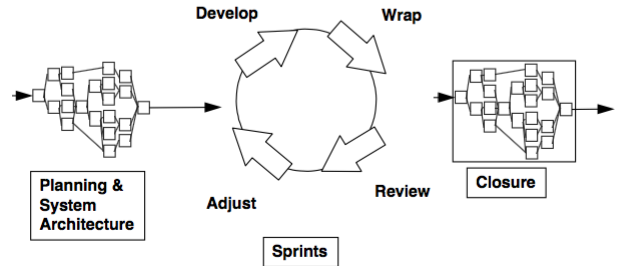
\includegraphics[width=0.6\textwidth]{scrum}
  	\caption{Scrum}
  \label{Figure:scrum}
\end{figure}


However, agile methods are not perfect by any means. For example: it is not always possible to make upfront cost estimation because of the volatile nature of development \cite{Ramesh:2010}. As always, an early architectural design decision may adversely affect future development. Despite these, I think it is preferable to take an agile approach to any modern mobile app development \cite{Wasserman:2010} because of the nature of the industry itself.

\section{Testing in Modern SE}
\label{sec:testing}

\subsection{Test Driven Development}

Test Driven Development (TDD) is a software engineering practice where automated unit tests are written before development. These tests fail at first, but start to pass as the development proceeds. Thus development itself remains focused and targeted \cite{Williams:2003}. It is also a part of Extreme Programming (XP). Modern agile teams believe that the advantages include \cite{George:2004} - 

\begin{itemize}
	\item Efficiency in error detection in later stages because of comprehensive development stage testing.
	\item Fast regression testing possible because of the test driven code.
	\item Testability (code that is easy to test) increases in the entire codebase.
	\item Loosely coupled system as a result of the need for mock objects.
\end{itemize}

However, some shortcomings of the TDD process are \cite{George:2004} - 

\begin{itemize}
	\item Some code is inherently difficult to unit test, for example: GUIs etc.
	\item The code must coherently support mock objects to isolate other code which proves hard in practice.
	\item Testing hard-to-test code needs a certain level of experience and determination.
\end{itemize}

In the literature, I have found TDD to be the current trend across the industry, including myself using the process in IBM during internship. However, TDD requires an experienced team in the required technology to implement the architecture and have a coherent data model. In short projects it can actually be counter productive.

\subsection{Behaviour Driven Development}

In TDD most developers are unsure what and how much to test, where to start etc. There is also usually a gulf between developer testing and customer acceptance. Behaviour Driven Development (BDD) attempts to answer these questions by mandating automated test cases based \textit{only} on the user stories \cite{Solis:2011}. Any other automated test is optional for the development teams. Below is a test structure for BDD, extracted from a user story - 

\begin{center}
\texttt{\textbf{Given} <init\_context>}\\
\texttt{\textbf{When} <event> occurs}\\
\texttt{\textbf{Then} <assert\_outcome>}
\end{center}

This style can be placed in between unit and integration tests in traditional testing. One major advantage is that it is easier to understand as a customer. BDD may or may not replace general unit testing itself. Also, regression testing mandatory as usual.